\documentclass[12pt]{article}
\usepackage{graphicx} % Required for inserting images
\usepackage{amsmath}
\usepackage{geometry}
\geometry{margin=1in}

\title{Population Econ HW1}
\author{YU HSIANG LIEN 1A202G34}
\date{November 2023}

\begin{document}

\maketitle

\section{Chapter 2}
\begin{enumerate}
    \item[\textbf{Q1}] 
    a. Size of labor force at the start of each year
    
    Y2008: $234 \times 0.662$ = 154.908m\\
    Y2012: $238 \times 0.642$ = 152.796m\\
    Y2016: $251 \times 0.627$ = 157.377m

    b. Officially unemployed population
    
    Y2008: $154.908 \times 0.05$ = 7.75m\\
    Y2012: $152.796 \times 0.091$ = 13.9m\\
    Y2016: $157.377 \times 0.049$ = 7.71m

    c. While it's true that the unemployment rate appeared lower in 2016 when compared to 2008, a closer examination reveals a significant drop in the labor participation rate by 4\% during this period. This decrease implies that there could be a substantial number of individuals who remain jobless but are not accounted for due to limitations in the data collection process. Consequently, when assessing such data, it becomes crucial not to underestimate the underlying issues concealed by the methodology of data collection.
    
    \item[\textbf{Q2}] 
    
    1. Charlie will ultimately choose more consumption.
       
    2. The steepness of the indifference curve guarantees this result since a steeper indifference curve means the person will value leisure more and thus work more and have more consumption. And since Charlie always requires more leisure than Larry to be equally happy when asked to forego a dollar of consumption. This means that Charlie has a higher marginal rate of substitution (MRS) between consumption and leisure compared to Larry. And thus Charlie will have a steeper indifference curve compared to Larry.
    
    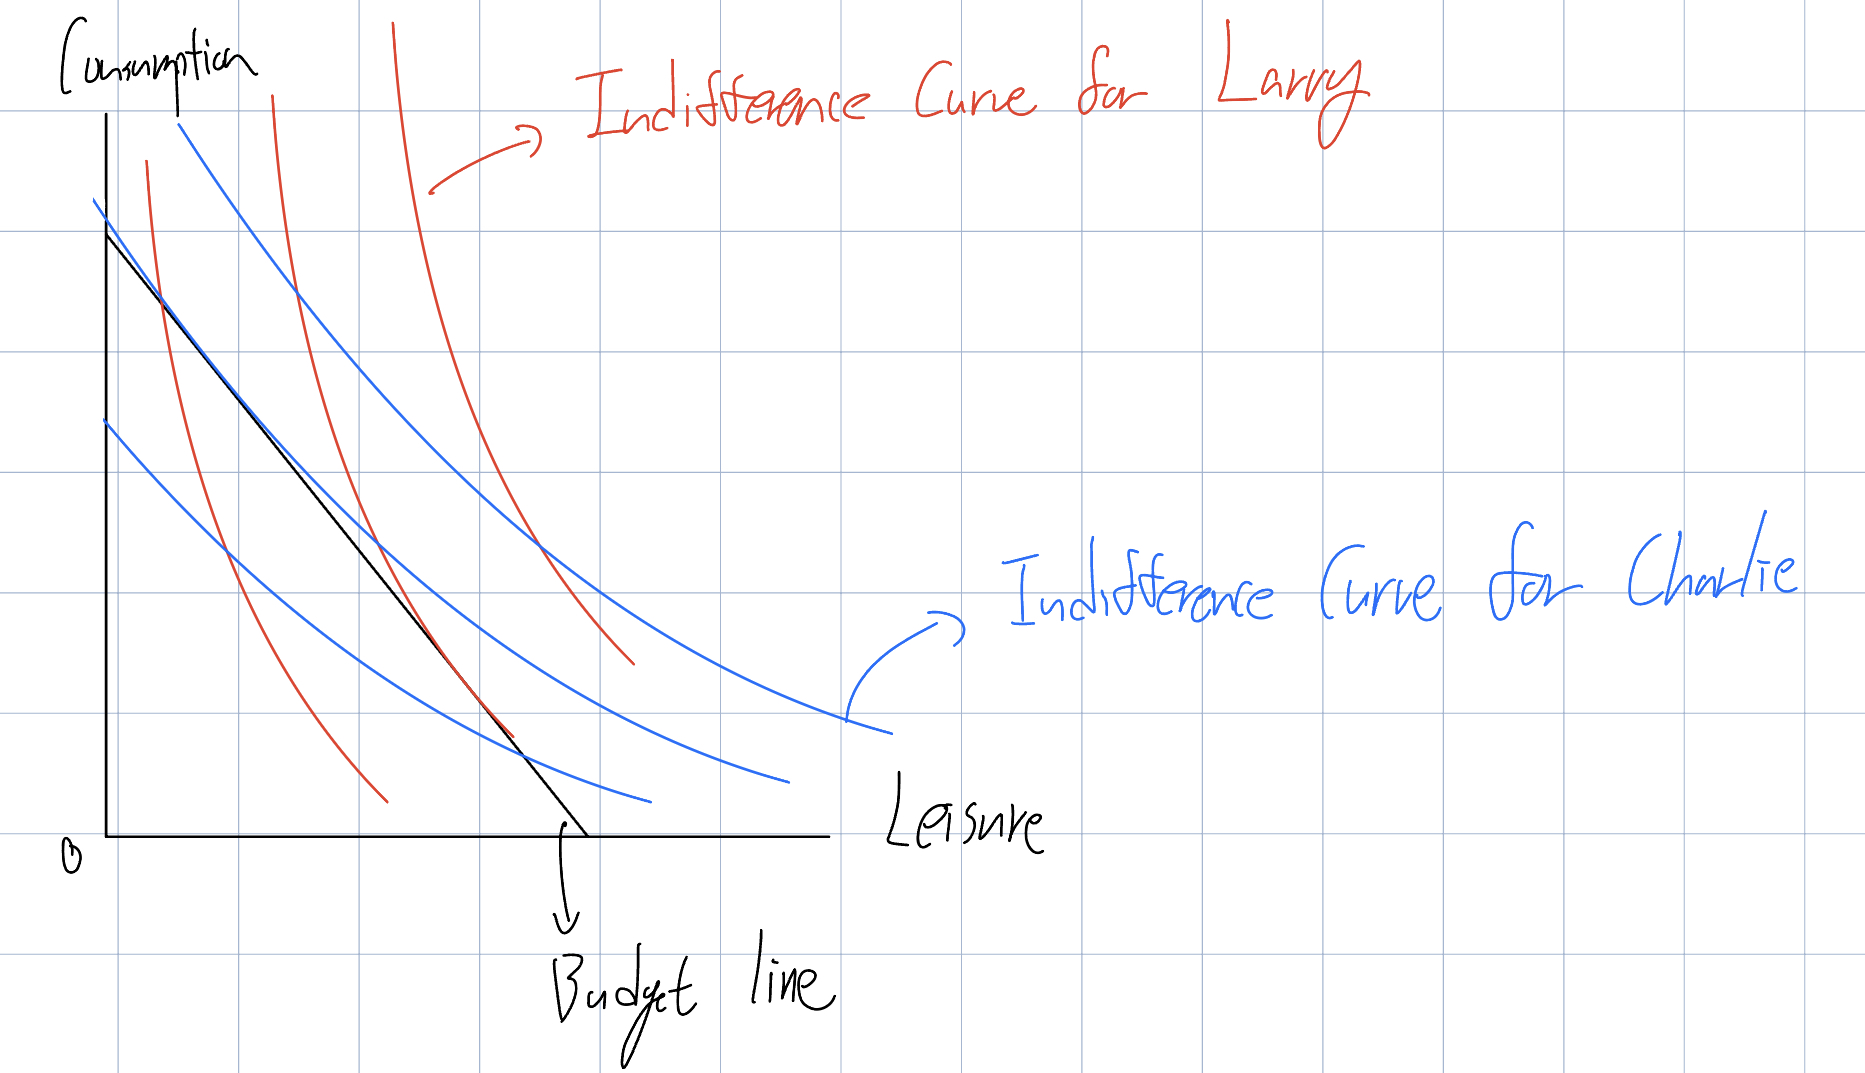
\includegraphics[width=0.9\linewidth]{截圖 2023-11-04 上午3.54.13.png}
        
    \item[\textbf{Q3}] 
    Non-labor income = 80\\
    Income for working up to 40 hrs: $((15 \times 0.8)-4)40 = 320$\\
    Income for working 40 to 110 hours: $((30 \times 0.8)-4)70 = 1400$
    
    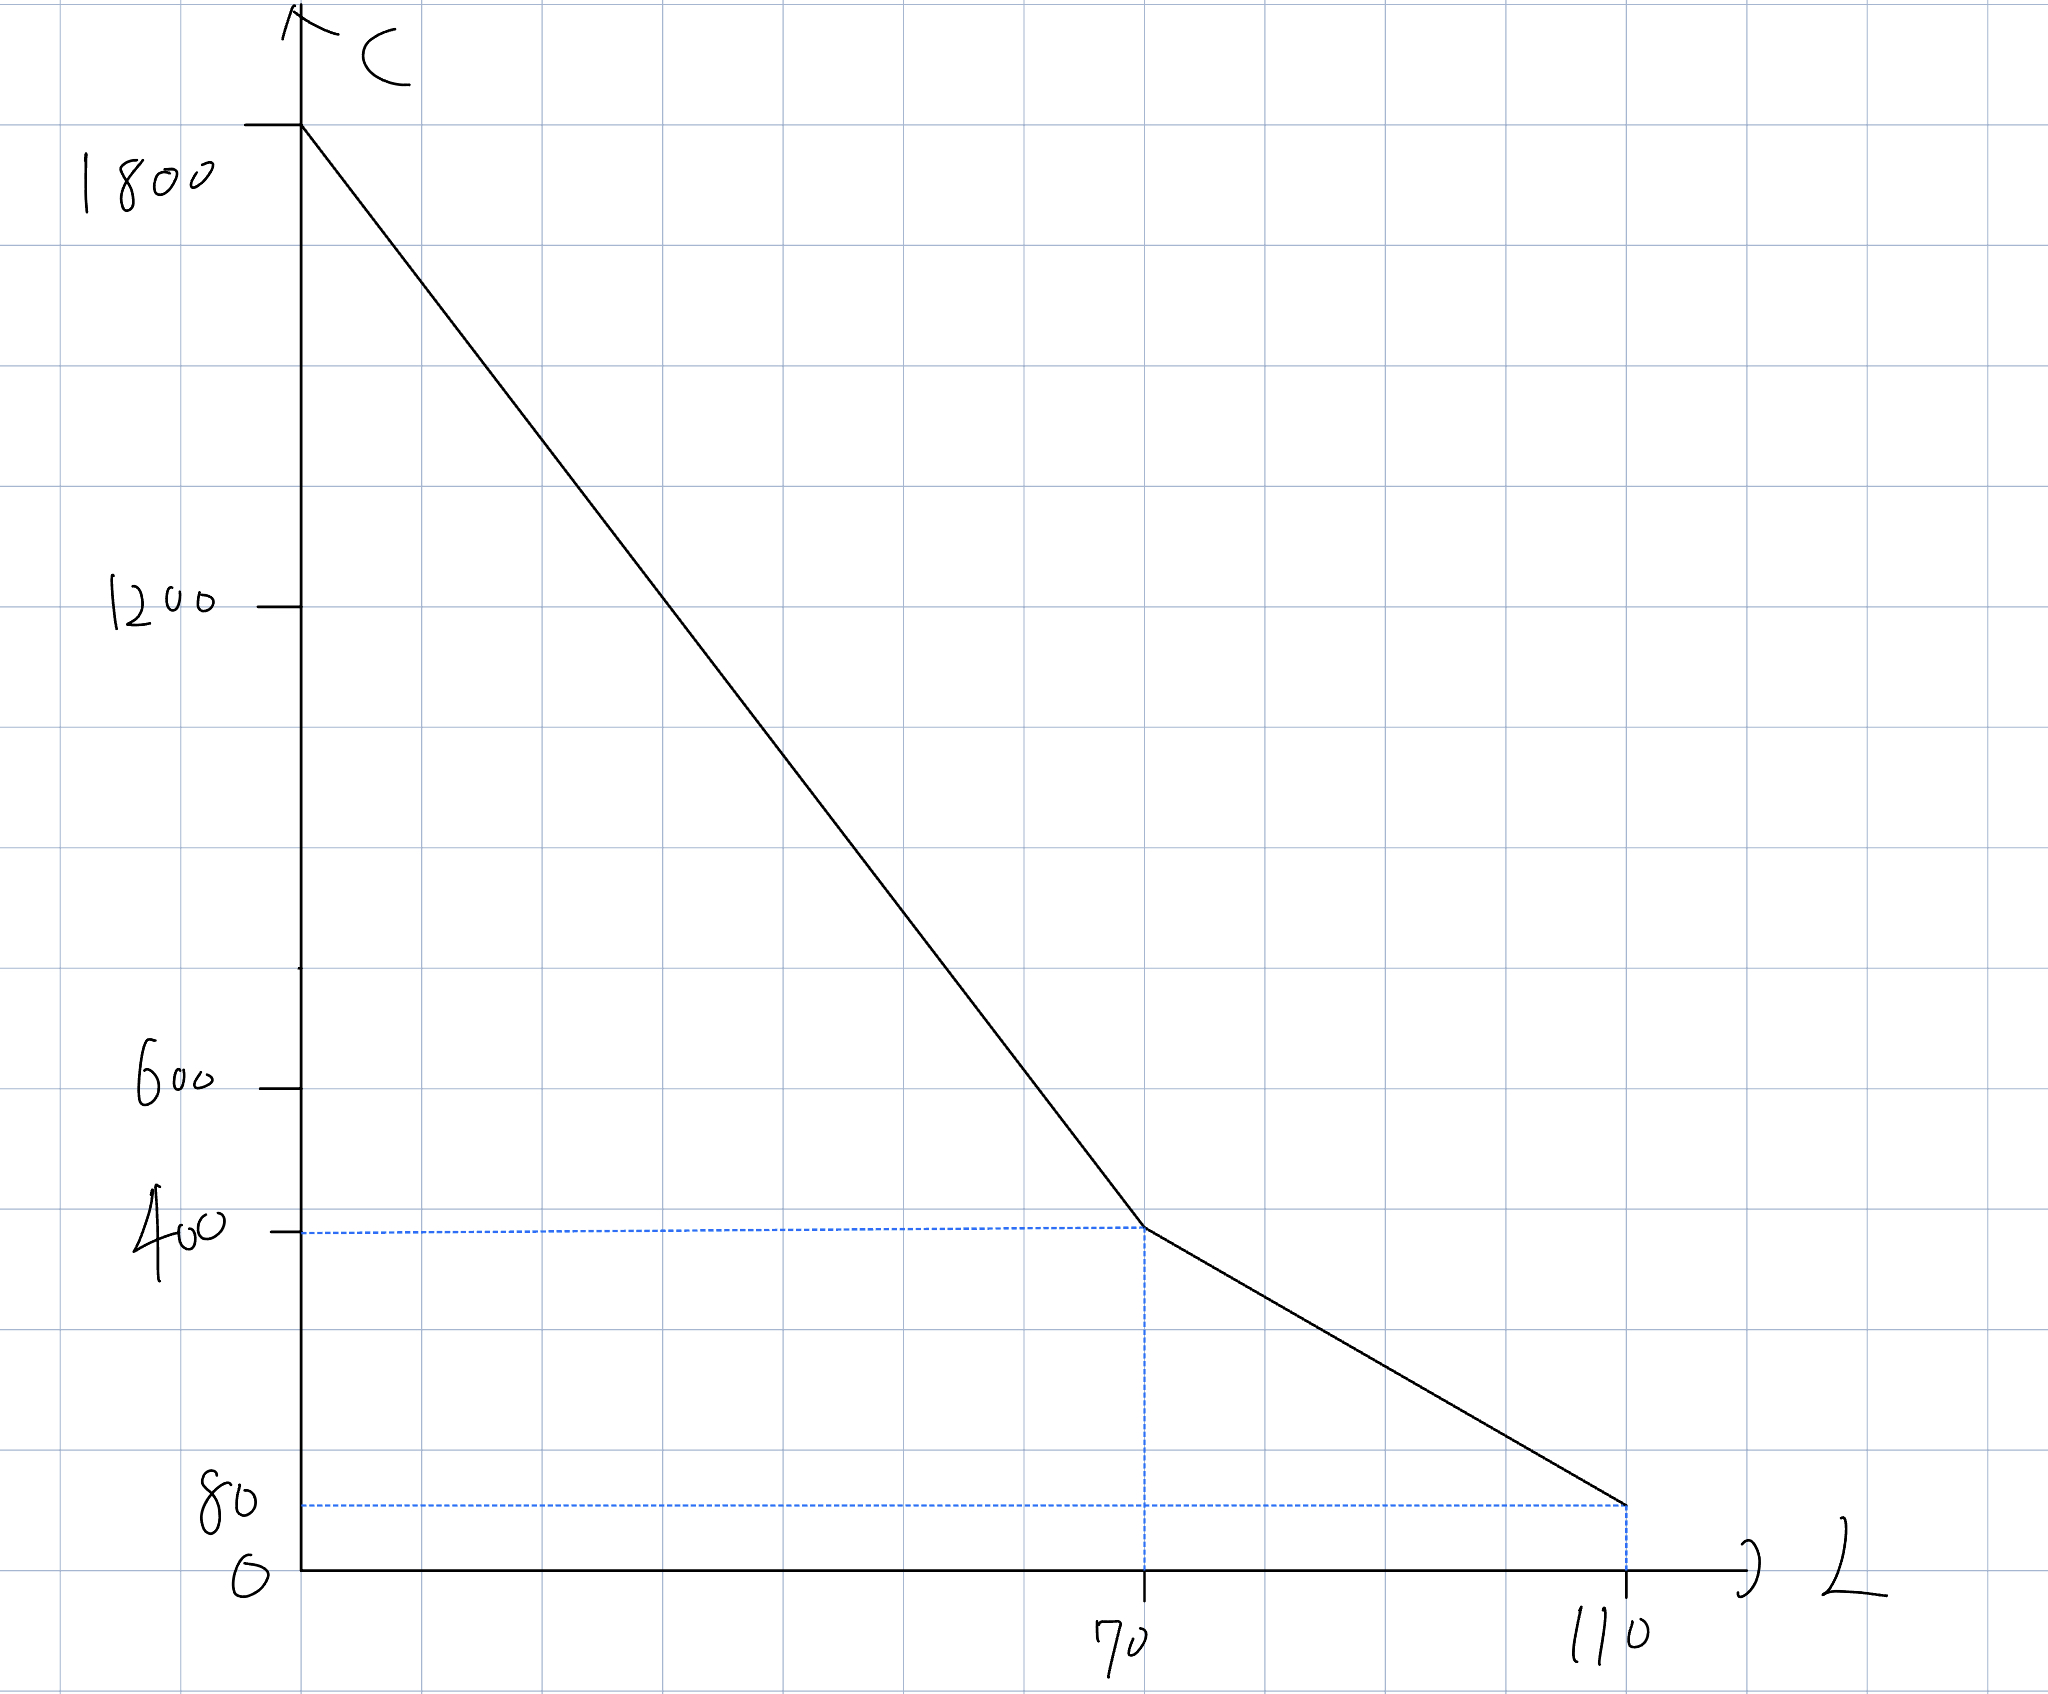
\includegraphics[width=0.8\linewidth]{截圖 2023-11-04 上午4.02.53.png}
        
    \item[\textbf{Q4}] 
    1. $U(C,L) = C \times L \Rightarrow MRS = \frac{MU_L}{MU_C} = \frac{C}{L}$ 
    
    2. Cindy's reservation wage $\Rightarrow$ MRS when not working at all $\Rightarrow \frac{660}{110} = 6$\\
    $\Rightarrow$ Reservation wage = $\$6$
    
    \item[\textbf{Q5}] 
    a. 
    \begin{align*} 
    110 \times 10 &=  1100 \\ 
    1100 + 320 &=  1420
    \end{align*}
    
    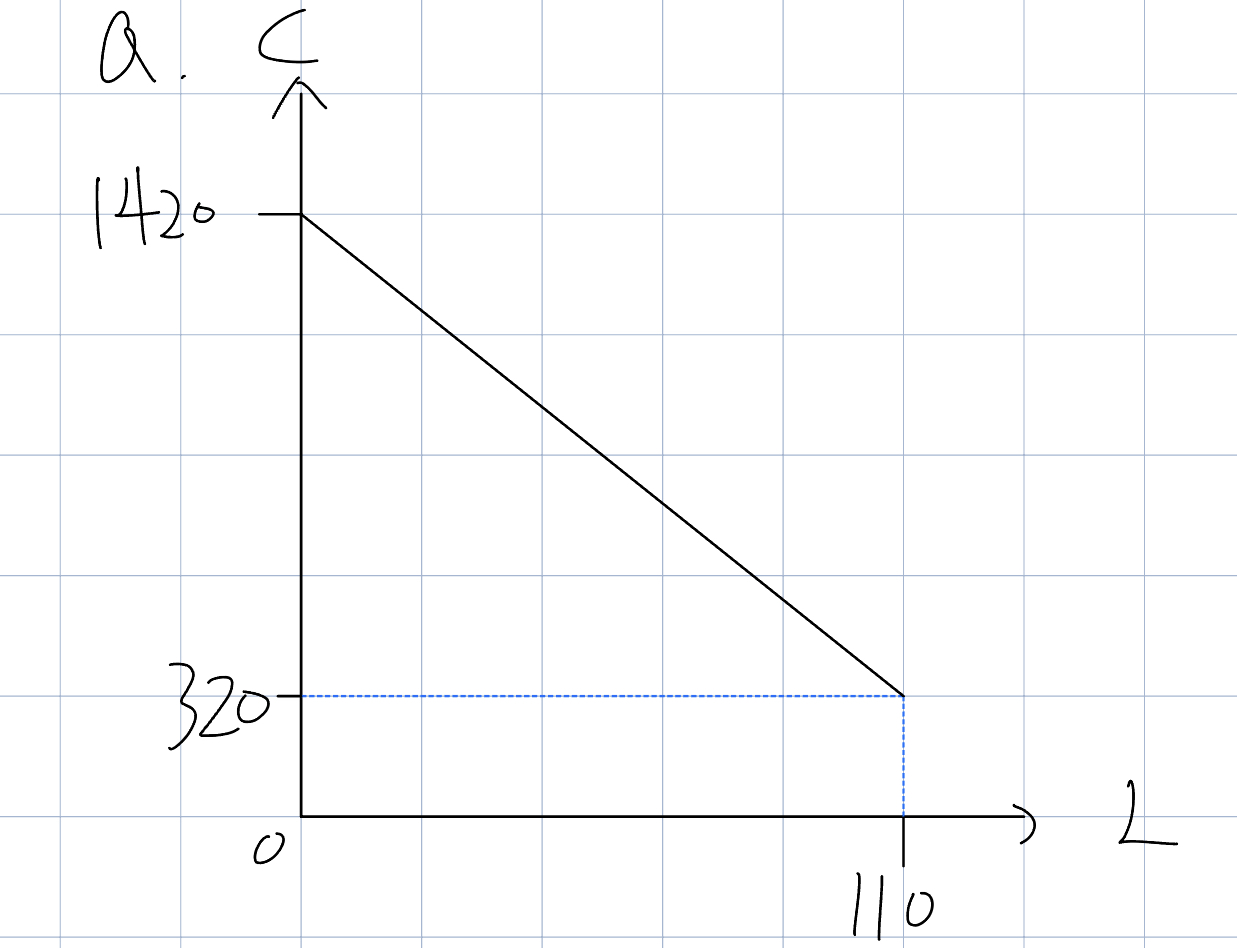
\includegraphics[width=1\linewidth]{IMG_E2C6480C7225-1.jpeg}

    b. MRS when L=100

    $MRS = \frac{MU_L}{MU_C} = \frac{C - 100}{L-40} = \frac{420 - 100}{100 - 40} = \frac{32}{6} = 5.33$

    c. Reservation wage

    $W_{RES} = \frac{320 - 100}{110-30} = \frac{22}{7} = \$3.14$

    d. Optimal consumption and leisure

    \begin{align*}
            MRS = w &\Rightarrow \frac{C - 100}{L - 40} = 10 \Rightarrow 10 = \frac{320 + 10(110 - L) -100}{L - 40}\\ &\Rightarrow 10L - 400 = 1320 - 10L \Rightarrow 20L = 1720\\
            &\Rightarrow L = 86\\
            &\Rightarrow C = 320 + 10(110 - 86) = 560
    \end{align*}

    $\Rightarrow Optimal (C,L) = (560, 86)$

    \item[\textbf{Q6}] 
    If a person's indifference curves between consumption and leisure are concave to the origin, the person A worker will either work all the time (Budget2) or will not work at all (Budget1). 

    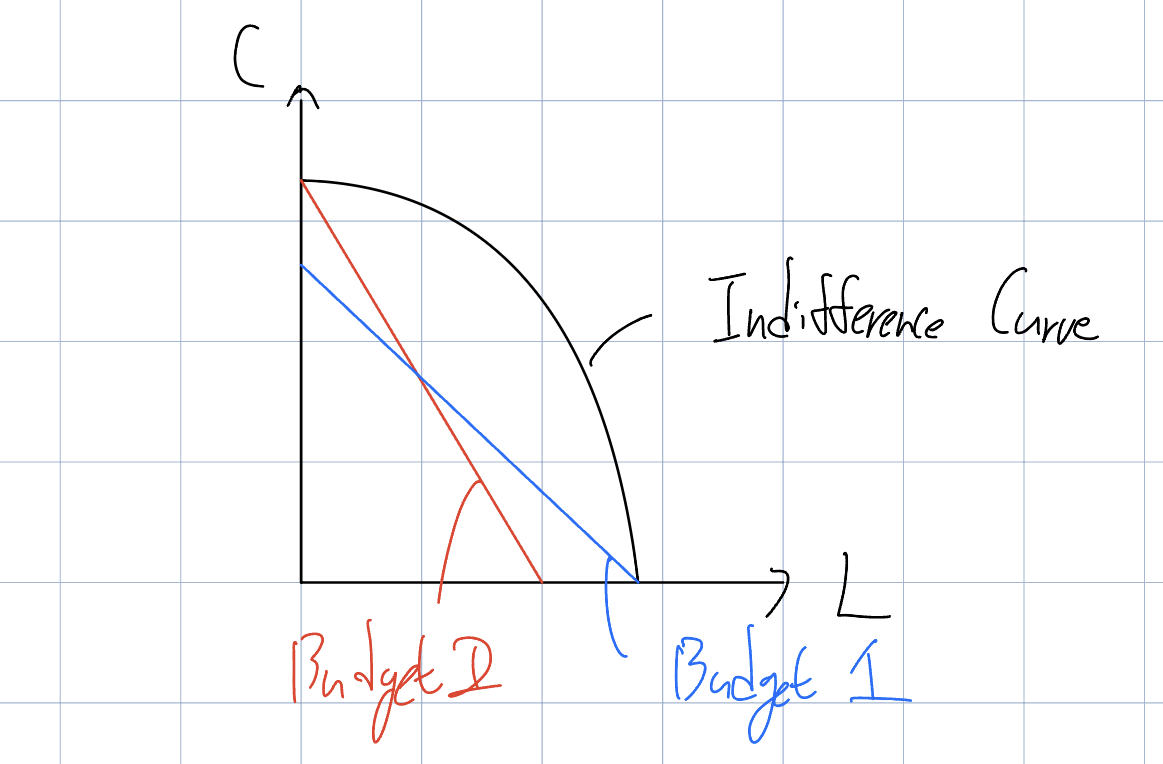
\includegraphics[width=0.75\linewidth]{IMG_6025608848EA-1.jpeg}
        
    \item[\textbf{Q7}] 
    a. Due to the identical wage progression and shared preferences among the workers, their lifetime patterns of working hours will remain consistent until an unexpected inheritance occurs. When Bill receives an inheritance, there is only an income effect and no substitution effect, so he is likely to work fewer hours (or at least not increase his hours) compared to Phil starting at the age of 35 and beyond.

    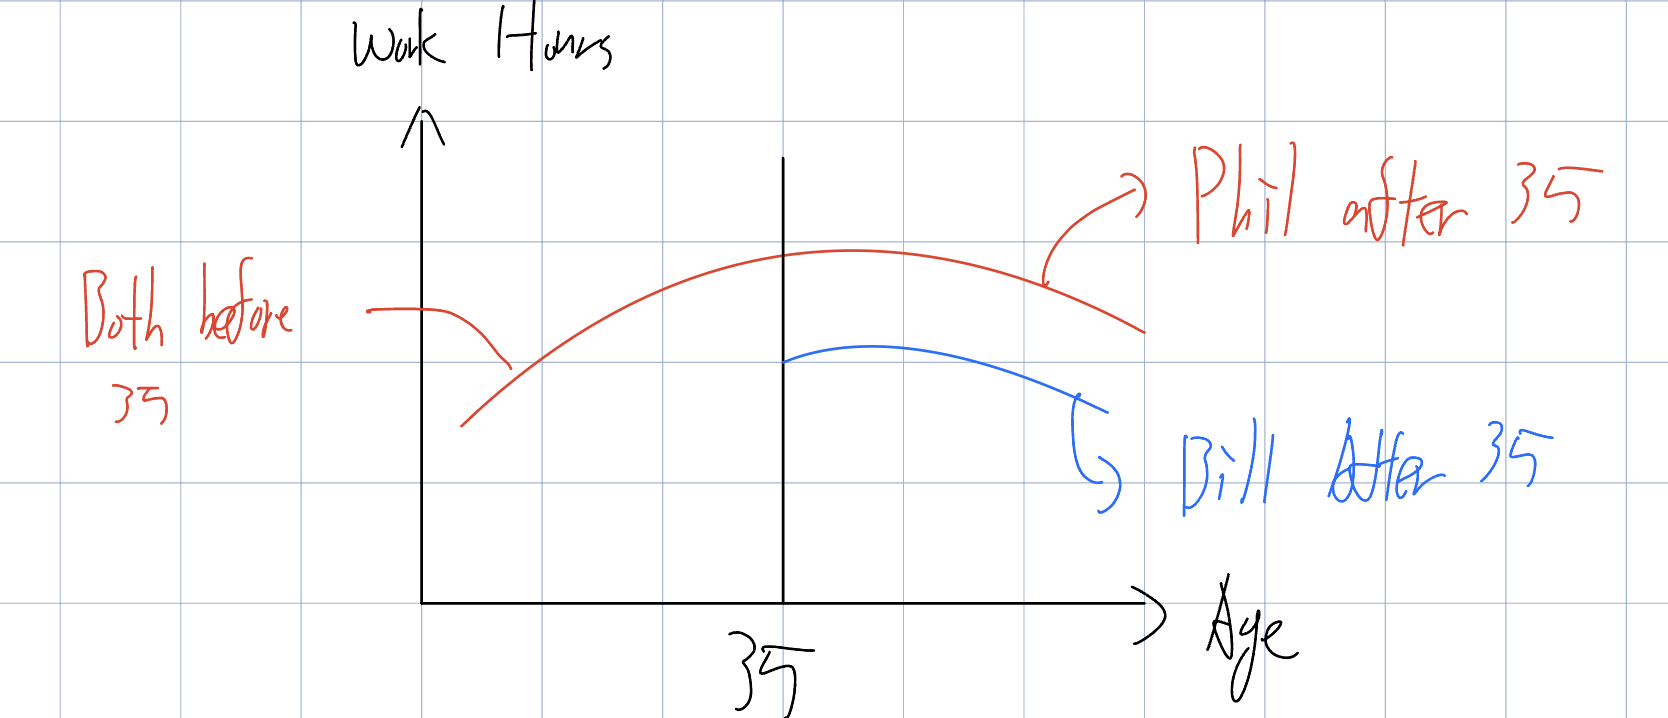
\includegraphics[width=0.75\linewidth]{IMG_81E7DB315363-1.jpeg}

    b. Since Bill always knows he is going to receive an inheritance, and so the inheritance will affect Bill by only income effect with no substitution effect, Bill will work fewer hours (or at least not more hours) than Phil over their entire life span.

    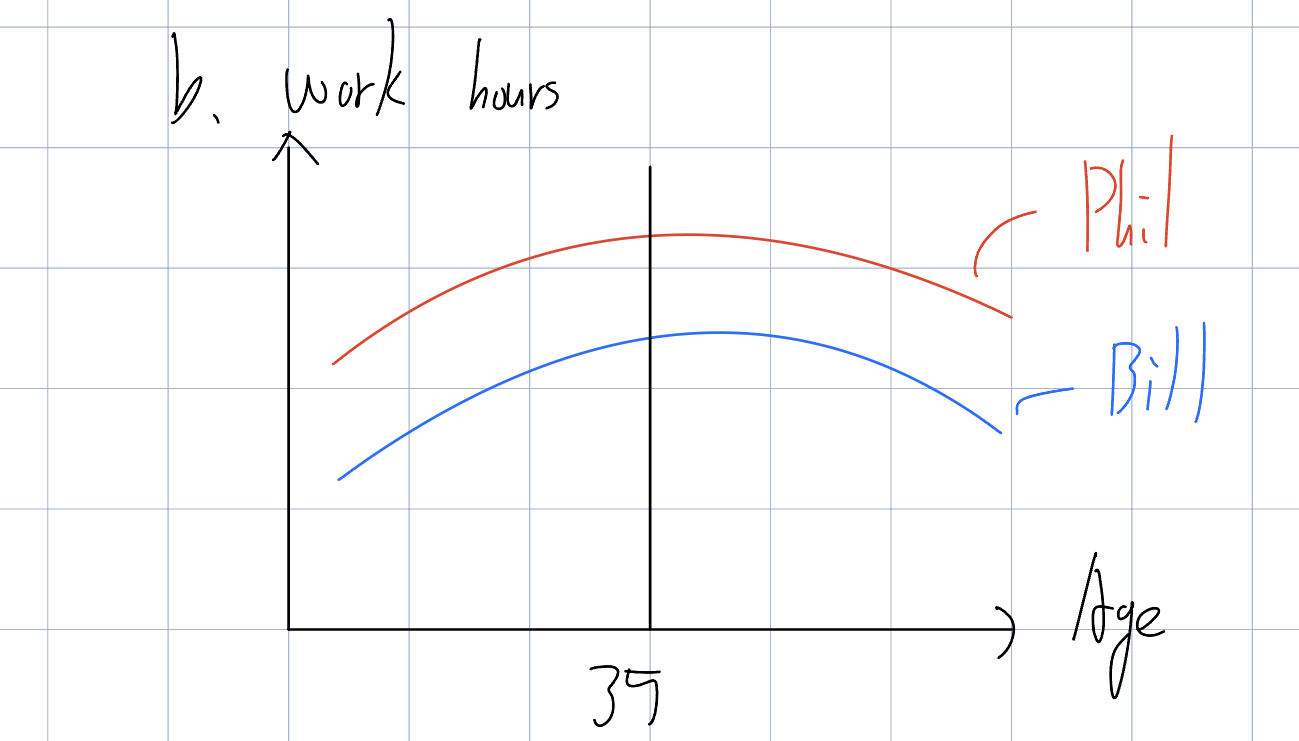
\includegraphics[width=0.75\linewidth]{IMG_D506A2FB645C-1.jpeg}

    \item[\textbf{Q8}] 
    a. If retirement benefits are fully adjusted for inflation, the announcement of higher inflation when the worker is 63 years old has no impact on the person's preferred retirement age. This is because, with full inflation adjustment, the person's calculations remain the same in real terms. The relative values of prices, wages, and retirement benefits do not change with or without inflation. Therefore, the individual faces an unchanged choice and their decision remains unaffected.

    b. In the case where retirement benefits are not fully adjusted for inflation, the announcement of higher inflation when the worker is 63 years old leads to a shift in the person's preferred retirement age. The reason is that without an inflation adjustment, the purchasing power of retirement benefits diminishes over time. If the individual chooses not to retire, they can maintain the same standard of living as they would have without inflation, as wages are assumed to fully compensate for inflation. However, if they retire at 65, their benefits have a lower real value due to inflation, making it insufficient to maintain their previous consumption level. As a result, their choice set for years of retirement and consumption is constrained below the original choice set before inflation, except for one point: not retiring at all. Therefore, if leisure and consumption are considered normal goods, both the income and substitution effects lead the individual to delay their retirement and work longer in life.
\end{enumerate}

\section{Chapter 3}
\begin{enumerate}
    \item[\textbf{Q1}]
    1. Since labor and capital are perfect substitutes in this case, the firm will choose the one that has a lower cost. So in the first case where capital cost per week is 750 and labor cost per week is $(300 \times 3) = 900$. The machine is cheaper, so the firm will choose a combination of all machines and no workers.

    2. In the second case here wage falls from 300 to 225. The cost of the machine is still 750, but the cost of workers is now $(225 \times 3) = 675$, which is lower. So since right now the cost of labor is lower and both inputs are perfect substitutes, the firm will have an input combination of all workers and no machine.

    3. The elasticity of labor demand as the wage falls from \$300 to \$225 will be negative infinity since when the wage decreases the input combination goes from 0 labor to all labor, thus we can conclude that the elasticity is $-\infty$.

    \item[\textbf{Q2}] 

    To find out in which firm the workers are more likely to organize and form a union, we can compare the elasticity of labor demand of both firms.

    Elasticity of Firm A
    $\Rightarrow \frac{(10000 - 20000)/20000}{(15 - 12)/12} = \frac{-1/2}{3/12} = -2$

    Elasticity of Firm B
    $\Rightarrow \frac{(33000 - 30000)/30000}{(15 - 20)/20} = \frac{-/10}{-1/4} = -0.4$ 

    So, with firm B's lower absolute elasticity of labor demand, we can conclude that workers in firm B are more likely to organize and form a union. When in a lower absolute elasticity condition, the workers will have more bargaining power when negotiating the wage and don't have to worry about that affecting employment, so workers in lower absolute elasticity of labor demand are more likely to form unions. And in this case, workers in firm B.

    \item[\textbf{Q3}] 
    a.  Effect of substitution effect: \\
    The substitution effect occurs when the relative prices of inputs change. In this case, when the prices change from w = 6 and r = 4 to w = 4 and r = 2, the relative price of labor (w/r) decreases from 1.5 to 2. This means that labor has become relatively cheaper compared to capital. In response to this price change, the firm will substitute more labor for capital, leading to an increase in the employment of labor and a decrease in the use of capital.
    
    b.  Effect of scale effect:\\
    The scale effect occurs when the overall cost of production changes due to price changes. In this case, when both the price of labor and capital decrease, the cost of production will generally decrease. When costs decrease, firms often choose to produce more, leading to an increase in employment of both labor and capital. This is because lower prices make it more cost-effective to use both inputs in larger quantities. So, the scale effect will result in an increase in both labor and capital usage.
    
    c.  Combined effect:\\
    The overall impact on labor and capital usage depends on the relative magnitude of the substitution effect and the scale effect. In this case, the substitution effect suggests an increase in labor usage and a decrease in capital usage, while the scale effect suggests an increase in both labor and capital usage. However, the net change in labor and capital usage cannot be conclusively determined without knowing the specific production function, technology, and the relative magnitudes of these effects. The final outcome will depend on the specific circumstances of the firm and its production process.\newpage
    
    \item[\textbf{Q4}] 

    The elasticity of labor demand = -0.4\\
    If wages increase by 5\%
    
    1. The change of the labor hired by the firm $\Rightarrow -0.4 \times 5\% = -2\%$
    
    
    $\Rightarrow$ The labor hired by the firm will decrease by $2\%$.

    2. When wages increase and labor that is hired decreases, it is likely that the marginal productivity of the last worker hired by the firm will increase. This is because the firm is hiring fewer workers, so the remaining workers may become more productive due to better resource allocation and more intensive use of labor.

    In summary, if the wage increases by 5 percent, the firm will hire 2 percent less labor, and the marginal productivity of the last worker hired will likely increase.

    \item[\textbf{Q5}] 
    Given the firm's technology, it's evident that a precise combination of 5 person-hours of labor and 3 machine-hours is necessary to yield 1 unit of output. This implies that labor and machine inputs are perfect complements. Consequently, alterations in the wage rate will have no impact on the labor input. Therefore, when wages increase from \$15 to \$20, the labor input remains constant, resulting in a short-run labor demand elasticity of 0.
    
    \item[\textbf{Q6}] 

    $E_S = 10 + W\\ E_D = 40 - 4W$

    a.\\ Equilibrium wage and employment:
    
    $10 + W = 40 - 2W \Rightarrow 5W = 30 \Rightarrow W = 6$

    $E = 40 - 24 \Rightarrow E = 16$

    $\Rightarrow$ Equilibrium (W, E) = (6, 16)

    Unemployment Rate = 16 - 16 / 16 = 0 

    $\Rightarrow$ Unemployment rate =0 \%

    b.\\ Impose minimum wage of \$8:

    $E_S = 10 + 8 = 18, E_D = 40 - 32 = 8$

    $16 - 8 = 8 \Rightarrow$ 8 workers will lose their job.

    $18 - 16 = 2 \Rightarrow$ 2 additional workers would want a job at the minimum wage.

    $\frac{18 - 8}{18} = \frac{5}{9} \Rightarrow$ The unemployment rate will be 5/9 (56\%)
    
    \item[\textbf{Q7}]

    w = \$10, price of each unit of K = 25, price of output = 50

    $f(E, K) = E^{1/2}K^{1/2}$

    a. $MP_L = \frac{1}{2}(E^{-1/2})(K^{1/2})$
    
    $\Rightarrow$ Marginal product of labor = $\frac{1}{2}(E^{-1/2})(K^{1/2})$

    b. Capital stock is fixed at 1,600 units

    Profit = $\pi(E) = (E^{1/2} \times 1600^{1/2})50 - 10E - 25 \times 1600 = 50(E^{1/2} \times 40) - 10E - 40000\\ = 2000E^{1/2} - 10E - 40000$
    
    To maximize profit $\frac{\partial \pi}{\partial E} = 0 \Rightarrow \frac{1}{2} \times 2000 \times E^{-1/2} - 10 = 0 \Rightarrow 1000E^{-1/2} = 10$
    
    $\Rightarrow E^{-1/2} = \frac{1}{100} \Rightarrow E = 10000$  

    Profit = $\pi = (10000^{1/2} \times 1600^{1/2})50 - 10 \times 10000 - 25 \times 1600$

    $= 100 \times 40 \times 50 - 100000 - 40000 = 200000 - 140000 = 60000$
    \newline 

    So, if the current capital stock is fixed at 1,600 units
    
    $\Rightarrow$ Firm should employ E = 10000, and the Profit $\pi$ = 60000
    

    This is for testing realtime refreash.
\end{enumerate}

\end{document}
